\vspace{1cm}
\section{{{\fontsize{17}{21}\selectfont \textbf{Results}}}}
\setlength{\columnsep}{1.5cm}
Here are the results obtained in camouflage object detection of RGB images.
\vspace{0.5cm}
\begin{figure}[h]
  \centering
  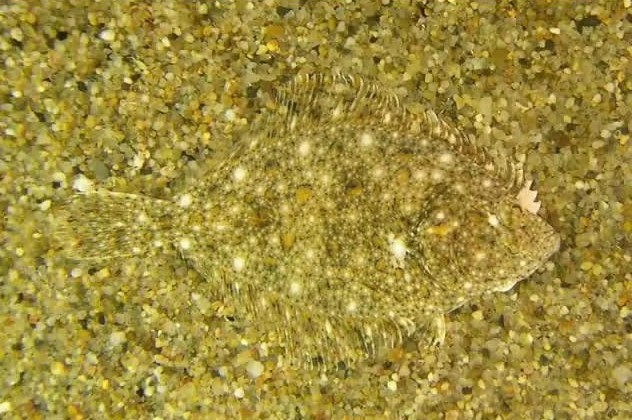
\includegraphics[width=0.9\textwidth,height=7cm]{sections/LBP/camourflage_00012.jpg}
  \caption{Camouflaged RGB image of fish}
  \label{fig:figure_label}
\end{figure}
\vspace{0.5cm}
\begin{figure}[h]
  \centering
  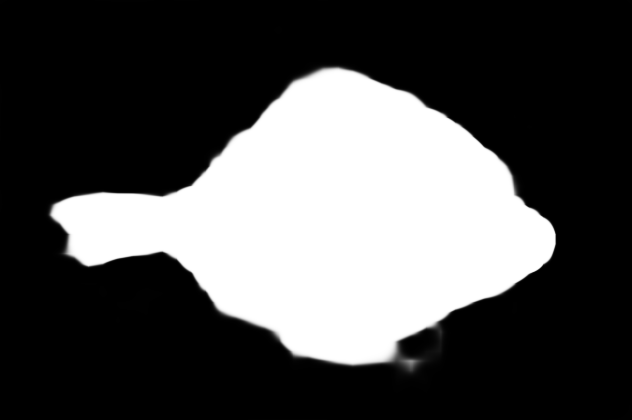
\includegraphics[width=0.9\textwidth,height=7cm]{sections/LBP/camourflage_00012.png}
  \caption{GT for the above RGB image}
  \label{fig:figure_label}
\end{figure}
\vspace{1cm}
\begin{figure}[h]
  \centering
  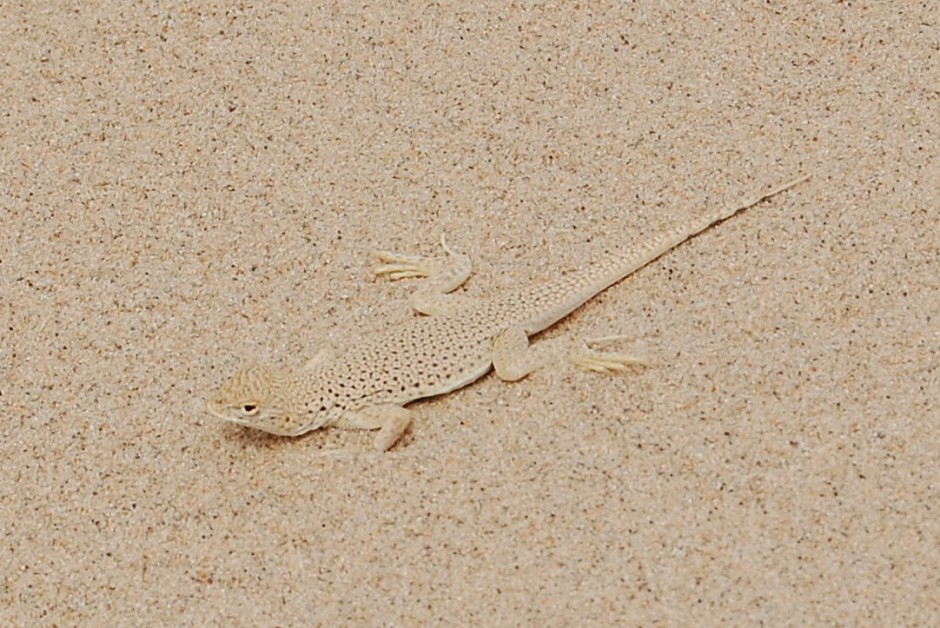
\includegraphics[width=0.9\textwidth,height=8cm]{sections/LBP/camourflage_00018.jpg}
  \caption{Camouflaged RGB Image}
  \label{fig:figure_label}
\end{figure}
\vspace{2cm}
\begin{figure}[h]
  \centering
  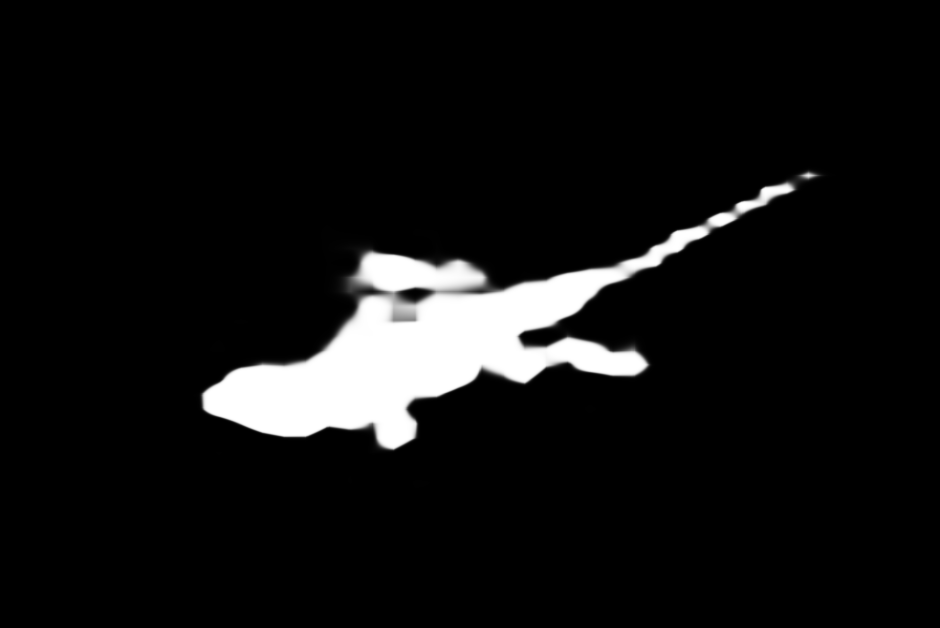
\includegraphics[width=0.9\textwidth,height=8cm]{sections/LBP/camourflage_00018.png}
  \caption{Grayscale output image}
  \label{fig:figure_label}
\end{figure}
\vspace{0.5cm}

\newpage
Below we present multi-spectral image consisting of 5-channelled image which is converted to 3-channelled image using feature extraction and data fusion.

\vspace{1cm}
\begin{figure}[h]
  \centering
  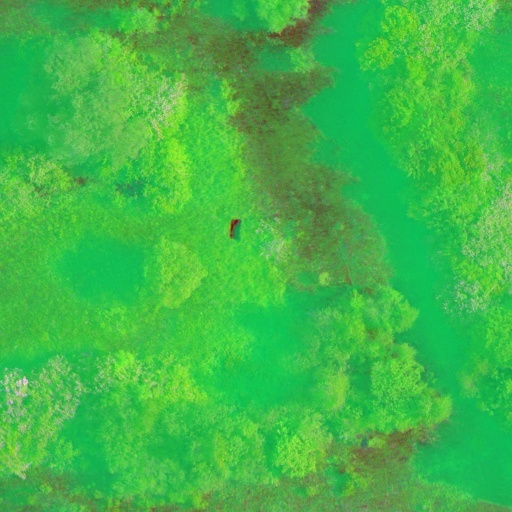
\includegraphics[width=0.9\textwidth,height=8cm]{sections/LBP/grass_0_rotated_0.jpg}
  \caption{MultiSpectral Image having a box like object at the center}
  \label{fig:figure_label}
\end{figure}
\vspace{2cm}

\begin{figure}[h]
  \centering
  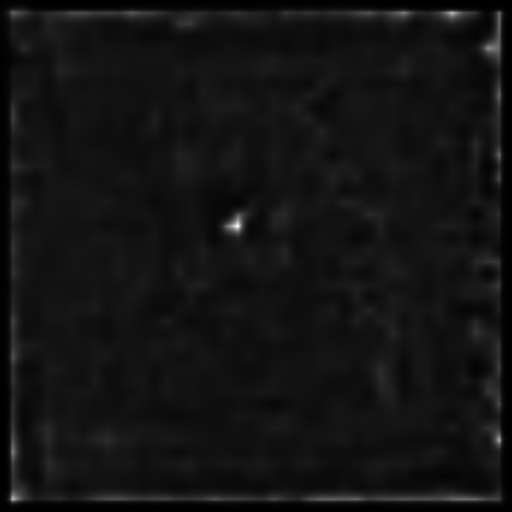
\includegraphics[width=0.9\textwidth,height=8cm]{sections/LBP/grass_0_rotated_0.png}
  \caption{Grayscale Output Image}
  \label{fig:figure_label}
\end{figure}
\vspace{0.5cm}
\newpage

\vspace{0.5cm}
\begin{figure}[h]
  \centering
  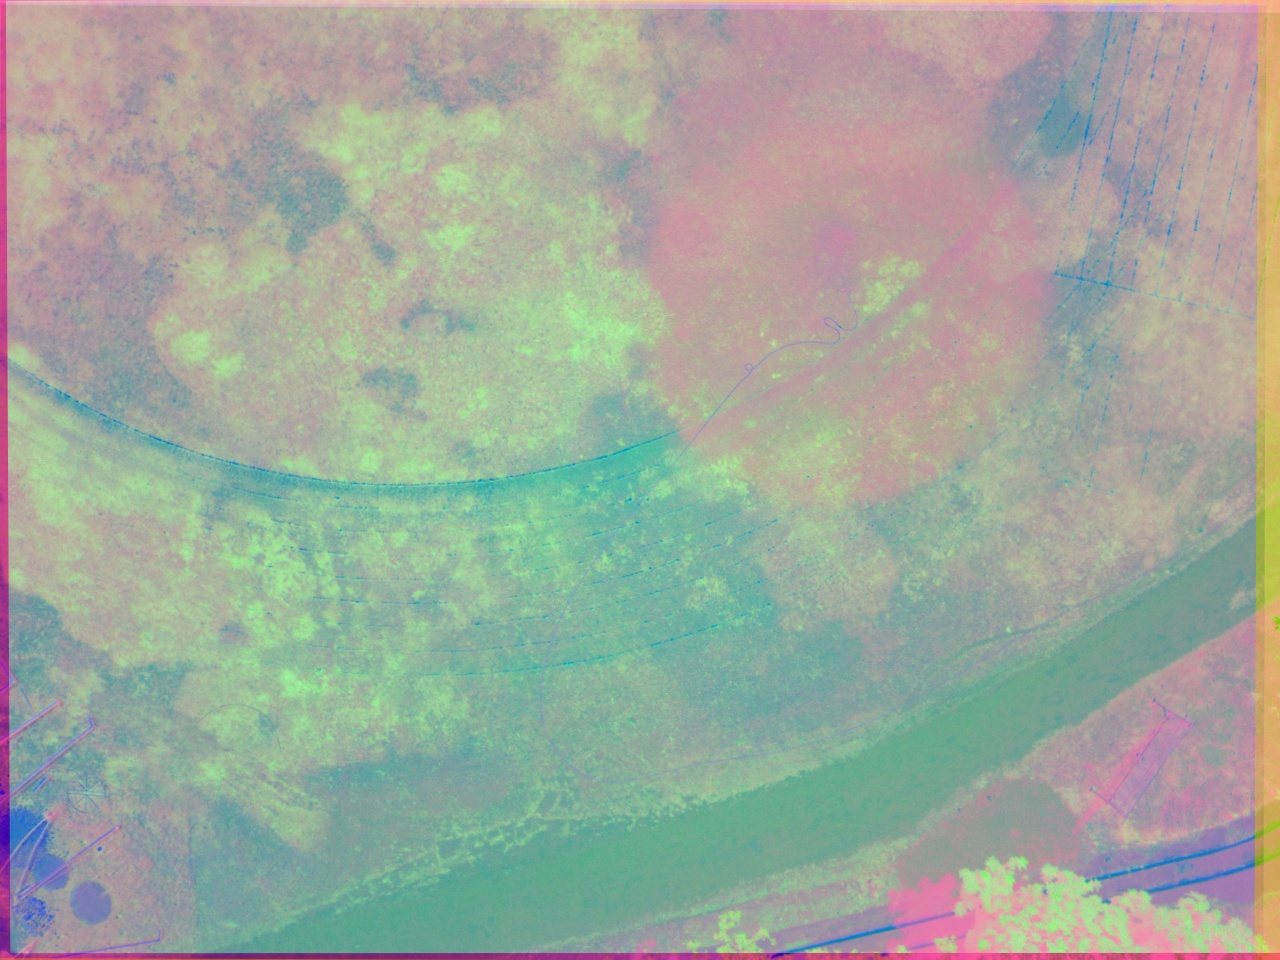
\includegraphics[width=0.9\textwidth,height=8cm]{sections/LBP/inp2.jpg}
  \caption{MultiSpectral data obtained using drone imaging}
  \label{fig:figure_label}
\end{figure}
\vspace{2cm}

\begin{figure}[h]
  \centering
  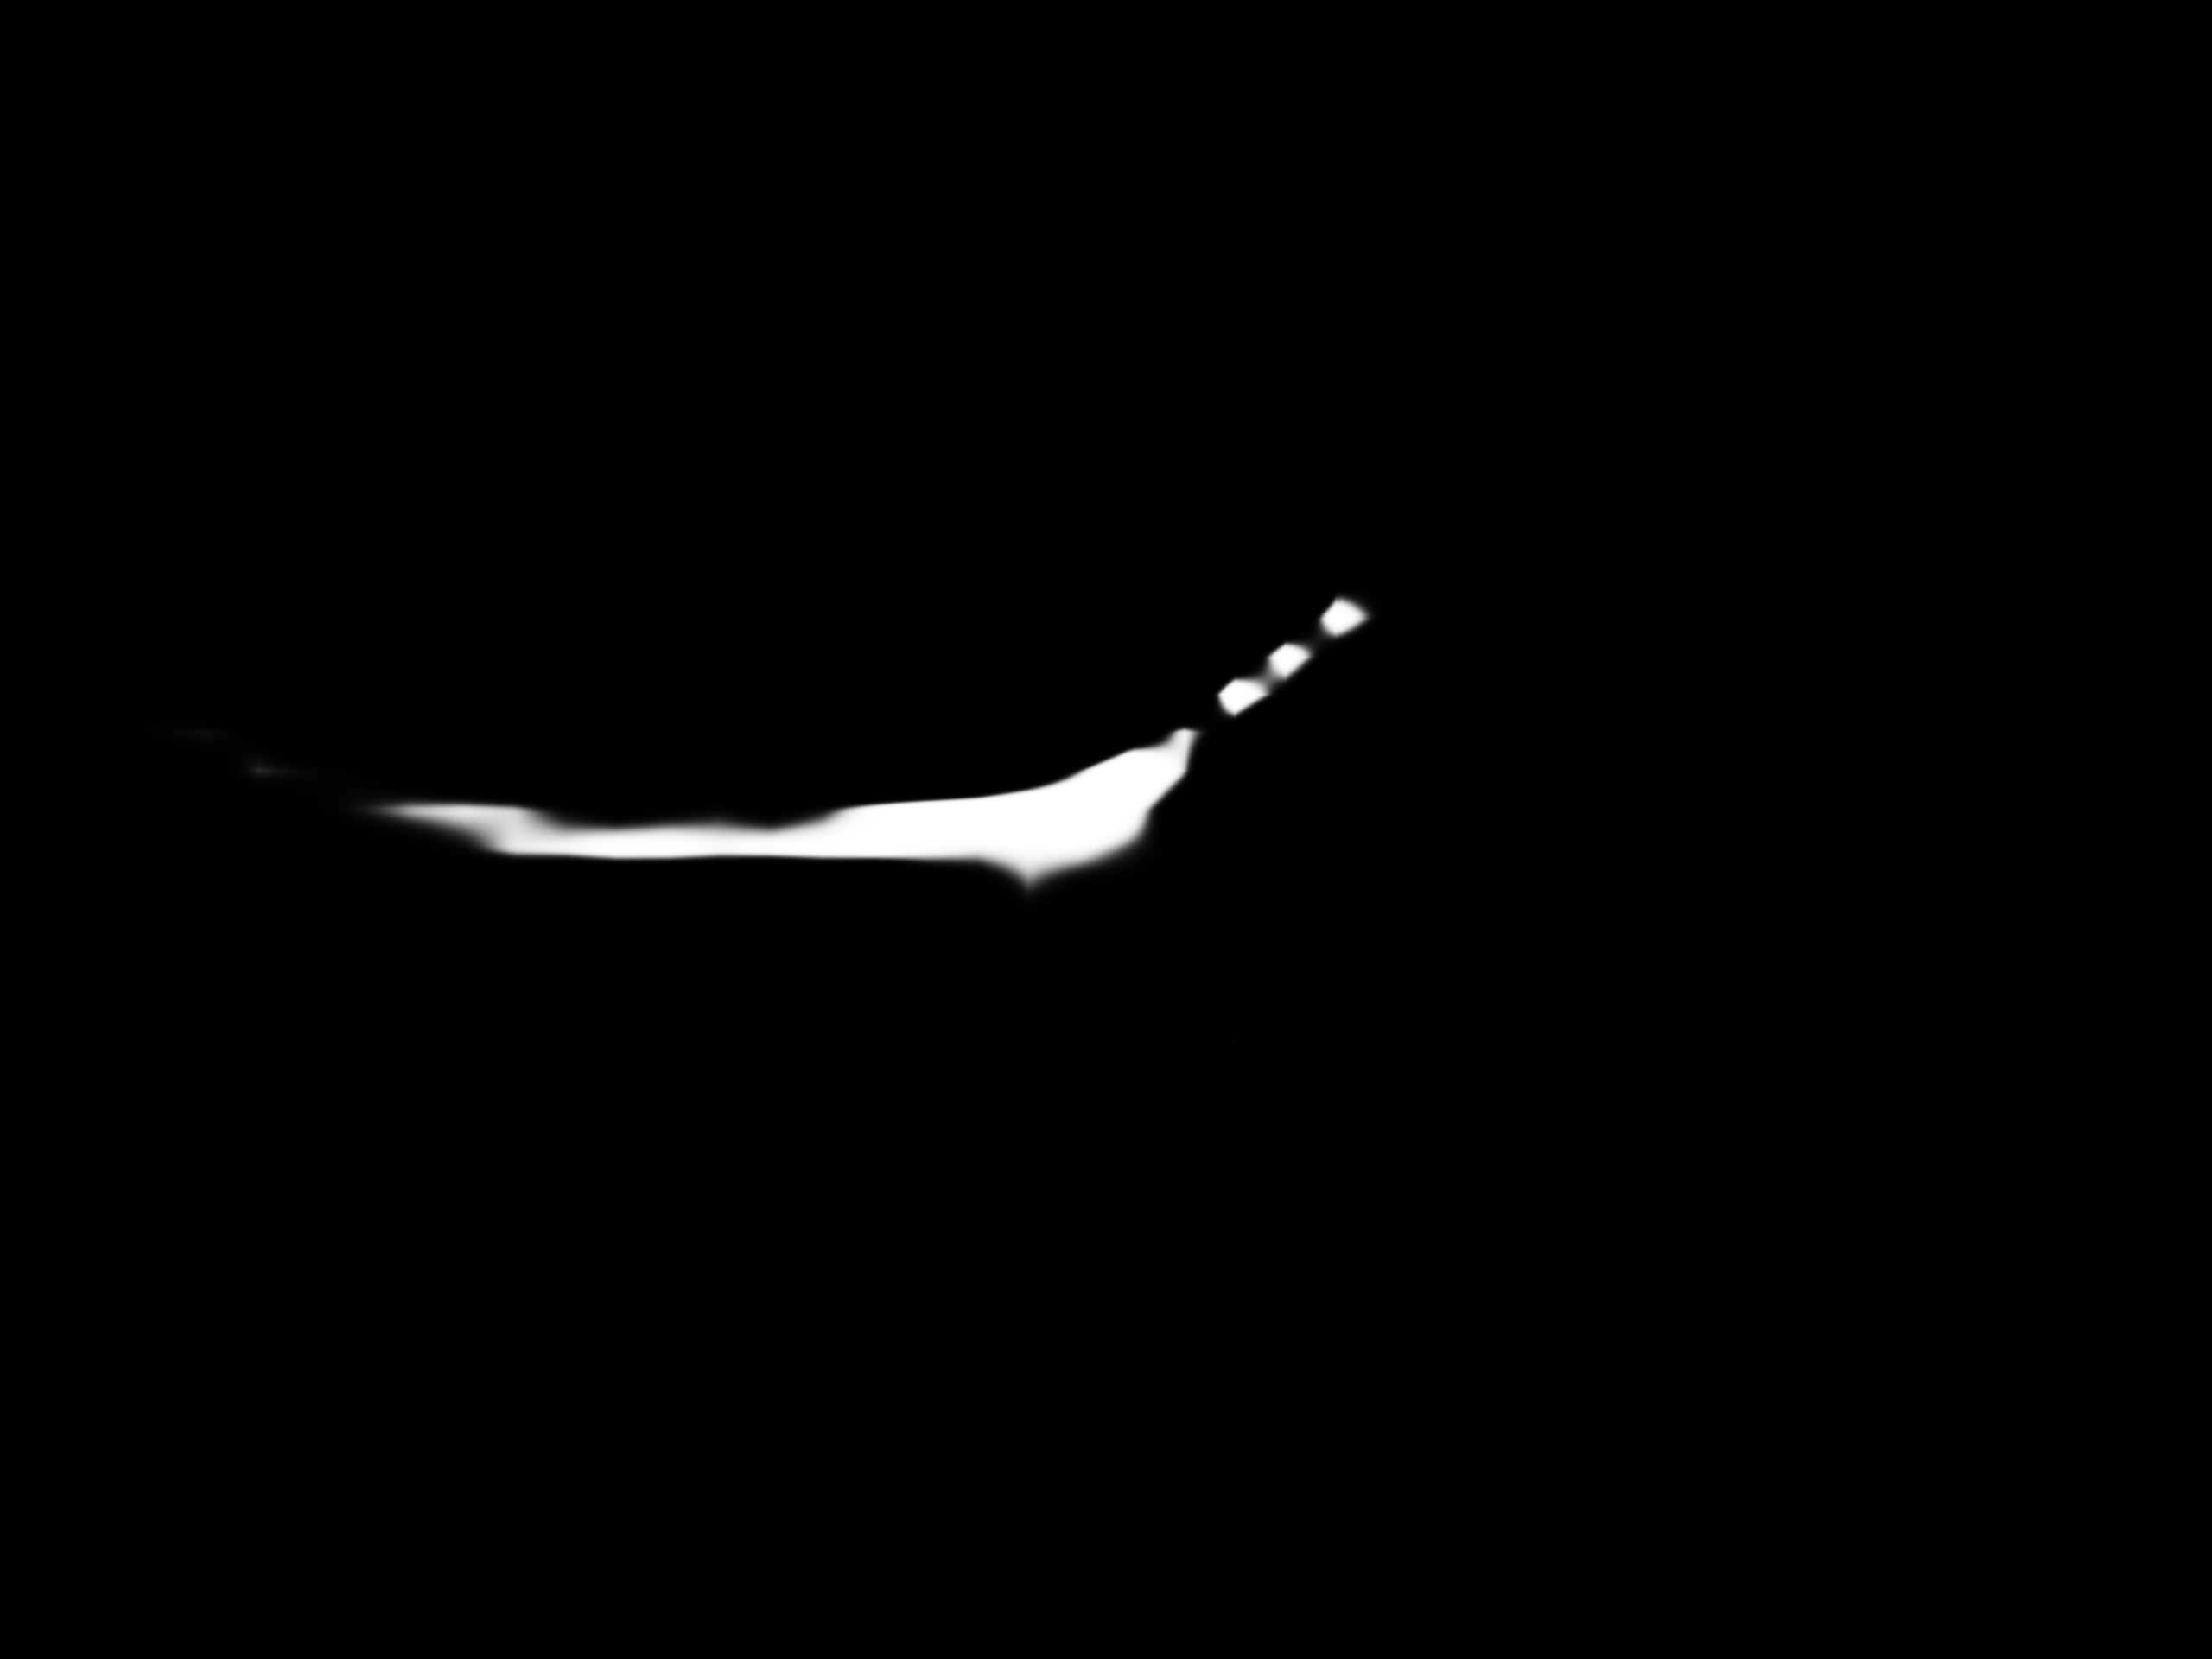
\includegraphics[width=0.9\textwidth,height=8cm]{sections/LBP/inp2.png}
  \caption{Grayscale Output Image}
  \label{fig:figure_label}
\end{figure}
\vspace{2cm}




\vspace{0.5cm}
{\color{gray}\hrule}
\vspace{0.5cm}


